%%%%%%%%%%%%%%%%%%%%%%%%%%%%%%%%%%%%%%%%%
% Beamer Presentation
% LaTeX Template
% Version 2.0 (March 8, 2022)
%
% This template originates from:
% https://www.LaTeXTemplates.com
%
% Author:
% Vel (vel@latextemplates.com)
%
% License:
% CC BY-NC-SA 4.0 (https://creativecommons.org/licenses/by-nc-sa/4.0/)
%
%%%%%%%%%%%%%%%%%%%%%%%%%%%%%%%%%%%%%%%%%

%----------------------------------------------------------------------------------------
%	PACKAGES AND OTHER DOCUMENT CONFIGURATIONS
%----------------------------------------------------------------------------------------

\documentclass[
	11pt, % Set the default font size, options include: 8pt, 9pt, 10pt, 11pt, 12pt, 14pt, 17pt, 20pt
	%t, % Uncomment to vertically align all slide content to the top of the slide, rather than the default centered
	%aspectratio=169, % Uncomment to set the aspect ratio to a 16:9 ratio which matches the aspect ratio of 1080p and 4K screens and projectors
]{beamer}

\graphicspath{{Images/}{./}} % Specifies where to look for included images (trailing slash required)

\usepackage{booktabs} % Allows the use of \toprule, \midrule and \bottomrule for better rules in tables

%----------------------------------------------------------------------------------------
%	SELECT LAYOUT THEME
%----------------------------------------------------------------------------------------

% Beamer comes with a number of default layout themes which change the colors and layouts of slides. Below is a list of all themes available, uncomment each in turn to see what they look like.

%\usetheme{default}
%\usetheme{AnnArbor}
%\usetheme{Antibes}
%\usetheme{Bergen}
%\usetheme{Berkeley}
%\usetheme{Berlin}
\usetheme{Boadilla} %me gusta
%\usetheme{CambridgeUS}
%\usetheme{Copenhagen}
%\usetheme{Darmstadt}
%\usetheme{Dresden}
%\usetheme{Frankfurt}
%\usetheme{Goettingen} %dos dos
%\usetheme{Hannover} %dos dos
%\usetheme{Ilmenau}
%\usetheme{JuanLesPins}
%\usetheme{Luebeck}
%\usetheme{Madrid}
%\usetheme{Malmoe}
%\usetheme{Marburg}
%\usetheme{Montpellier}
%\usetheme{PaloAlto}
%\usetheme{Pittsburgh}
%\usetheme{Rochester} %muy flat
%\usetheme{Singapore}
%\usetheme{Szeged}
%\usetheme{Warsaw}

%----------------------------------------------------------------------------------------
%	SELECT COLOR THEME
%----------------------------------------------------------------------------------------

% Beamer comes with a number of color themes that can be applied to any layout theme to change its colors. Uncomment each of these in turn to see how they change the colors of your selected layout theme.

%\usecolortheme{albatross}
%\usecolortheme{beaver}
%\usecolortheme{beetle}
%\usecolortheme{crane}
%\usecolortheme{dolphin}
%\usecolortheme{dove}
%\usecolortheme{fly}
%\usecolortheme{lily} %default
%\usecolortheme{monarca}
%\usecolortheme{seagull}
%\usecolortheme{seahorse}
%\usecolortheme{spruce}
%\usecolortheme{whale}
%\usecolortheme{wolverine}

%----------------------------------------------------------------------------------------
%	SELECT FONT THEME & FONTS
%----------------------------------------------------------------------------------------

% Beamer comes with several font themes to easily change the fonts used in various parts of the presentation. Review the comments beside each one to decide if you would like to use it. Note that additional options can be specified for several of these font themes, consult the beamer documentation for more information.

\usefonttheme{default} % Typeset using the default sans serif font
%\usefonttheme{serif} % Typeset using the default serif font (make sure a sans font isn't being set as the default font if you use this option!)
%\usefonttheme{structurebold} % Typeset important structure text (titles, headlines, footlines, sidebar, etc) in bold
%\usefonttheme{structureitalicserif} % Typeset important structure text (titles, headlines, footlines, sidebar, etc) in italic serif
%\usefonttheme{structuresmallcapsserif} % Typeset important structure text (titles, headlines, footlines, sidebar, etc) in small caps serif

%------------------------------------------------

%\usepackage{mathptmx} % Use the Times font for serif text
\usepackage{palatino} % Use the Palatino font for serif text

\usepackage[ruled,vlined]{algorithm2e}
%\usepackage{helvet} % Use the Helvetica font for sans serif text
\usepackage[default]{opensans} % Use the Open Sans font for sans serif text
\usepackage[spanish]{babel}
%\usepackage[default]{FiraSans} % Use the Fira Sans font for sans serif text
%\usepackage[default]{lato} % Use the Lato font for sans serif text

%----------------------------------------------------------------------------------------
%	SELECT INNER THEME
%----------------------------------------------------------------------------------------

% Inner themes change the styling of internal slide elements, for example: bullet points, blocks, bibliography entries, title pages, theorems, etc. Uncomment each theme in turn to see what changes it makes to your presentation.

%\useinnertheme{default}
\useinnertheme{circles}
%\useinnertheme{rectangles}
%\useinnertheme{rounded}
%\useinnertheme{inmargin}

%----------------------------------------------------------------------------------------
%	SELECT OUTER THEME
%----------------------------------------------------------------------------------------

% Outer themes change the overall layout of slides, such as: header and footer lines, sidebars and slide titles. Uncomment each theme in turn to see what changes it makes to your presentation.

%\useoutertheme{default}
%\useoutertheme{infolines}
%\useoutertheme{miniframes}
%\useoutertheme{smoothbars}
%\useoutertheme{sidebar}
%\useoutertheme{split}
%\useoutertheme{shadow}
%\useoutertheme{tree}
%\useoutertheme{smoothtree}

%\setbeamertemplate{footline} % Uncomment this line to remove the footer line in all slides
%\setbeamertemplate{footline}[page number] % Uncomment this line to replace the footer line in all slides with a simple slide count

%\setbeamertemplate{navigation symbols}{} % Uncomment this line to remove the navigation symbols from the bottom of all slides

%----------------------------------------------------------------------------------------
%	PRESENTATION INFORMATION
%----------------------------------------------------------------------------------------

\title[SEMINARIO DE INVESTIGACIÓN I]{Estrategias para la exploración coordinada multi-VANT} % The short title in the optional parameter appears at the bottom of every slide, the full title in the main parameter is only on the title page

%\subtitle{Optional Subtitle} % Presentation subtitle, remove this command if a subtitle isn't required

\author[Luis Ballado]{Luis Ballado} % Presenter name(s), the optional parameter can contain a shortened version to appear on the bottom of every slide, while the main parameter will appear on the title slide

\institute[CINVESTAV]{CINVESTAV - UNIDAD TAMAULIPAS \\ \smallskip \textit{luis.ballado@cinvestav.mx}} % Your institution, the optional parameter can be used for the institution shorthand and will appear on the bottom of every slide after author names, while the required parameter is used on the title slide and can include your email address or additional information on separate lines

\date[\today]{\today} % Presentation date or conference/meeting name, the optional parameter can contain a shortened version to appear on the bottom of every slide, while the required parameter value is output to the title slide

%----------------------------------------------------------------------------------------

\begin{document}

%----------------------------------------------------------------------------------------
%	TITLE SLIDE
%----------------------------------------------------------------------------------------

\begin{frame}
	\titlepage % Output the title slide, automatically created using the text entered in the PRESENTATION INFORMATION block above
\end{frame}

%----------------------------------------------------------------------------------------
%	TABLE OF CONTENTS SLIDE
%----------------------------------------------------------------------------------------

% The table of contents outputs the sections and subsections that appear in your presentation, specified with the standard \section and \subsection commands. You may either display all sections and subsections on one slide with \tableofcontents, or display each section at a time on subsequent slides with \tableofcontents[pausesections]. The latter is useful if you want to step through each section and mention what you will discuss.

%\begin{frame}
%	\frametitle{Contenido} % Slide title, remove this command for no title
	
%	\tableofcontents % Output the table of contents (all sections on one slide)
	%\tableofcontents[pausesections] % Output the table of contents (break sections up across separate slides)
%\end{frame}

%----------------------------------------------------------------------------------------
%	PRESENTATION BODY SLIDES
%----------------------------------------------------------------------------------------

%\section{Introducción} % Sections are added in order to organize your presentation into discrete blocks, all sections and subsections are automatically output to the table of contents as an overview of the talk but NOT output in the presentation as separate slides

%------------------------------------------------

\begin{frame}

  En la última década el uso de los Vehículos Aéreos No Tripulados (VANTs) ha tenido mucho auge y sus aplicaciones van en aumento.

  \begin{figure}[h]
    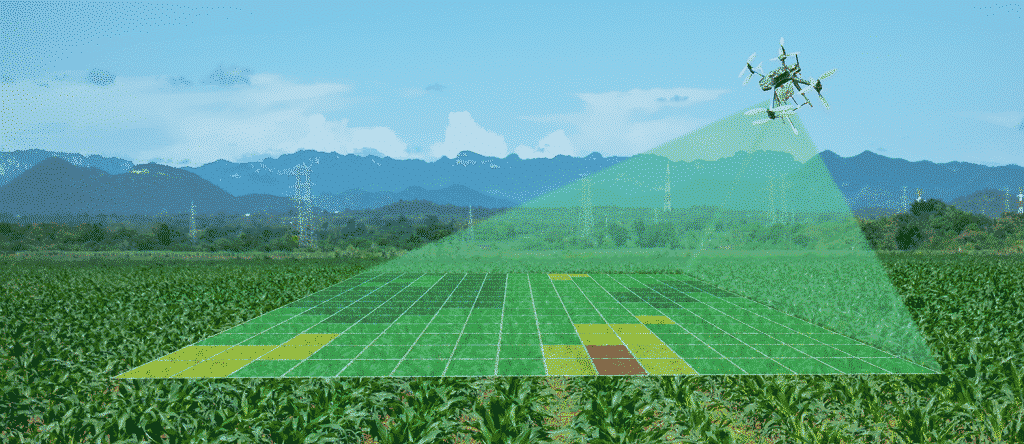
\includegraphics[width=0.7\linewidth]{drone_altura}
  \end{figure}

  Siendo la perspectiva privilegiada una de las principales ventajas.
  
\end{frame}

\begin{frame}

  Dentro de la robótica móvil y aérea se tienen problemas en común, uno de estos es la exploración de zonas desconocidas. 
  
  \begin{figure}[h]
    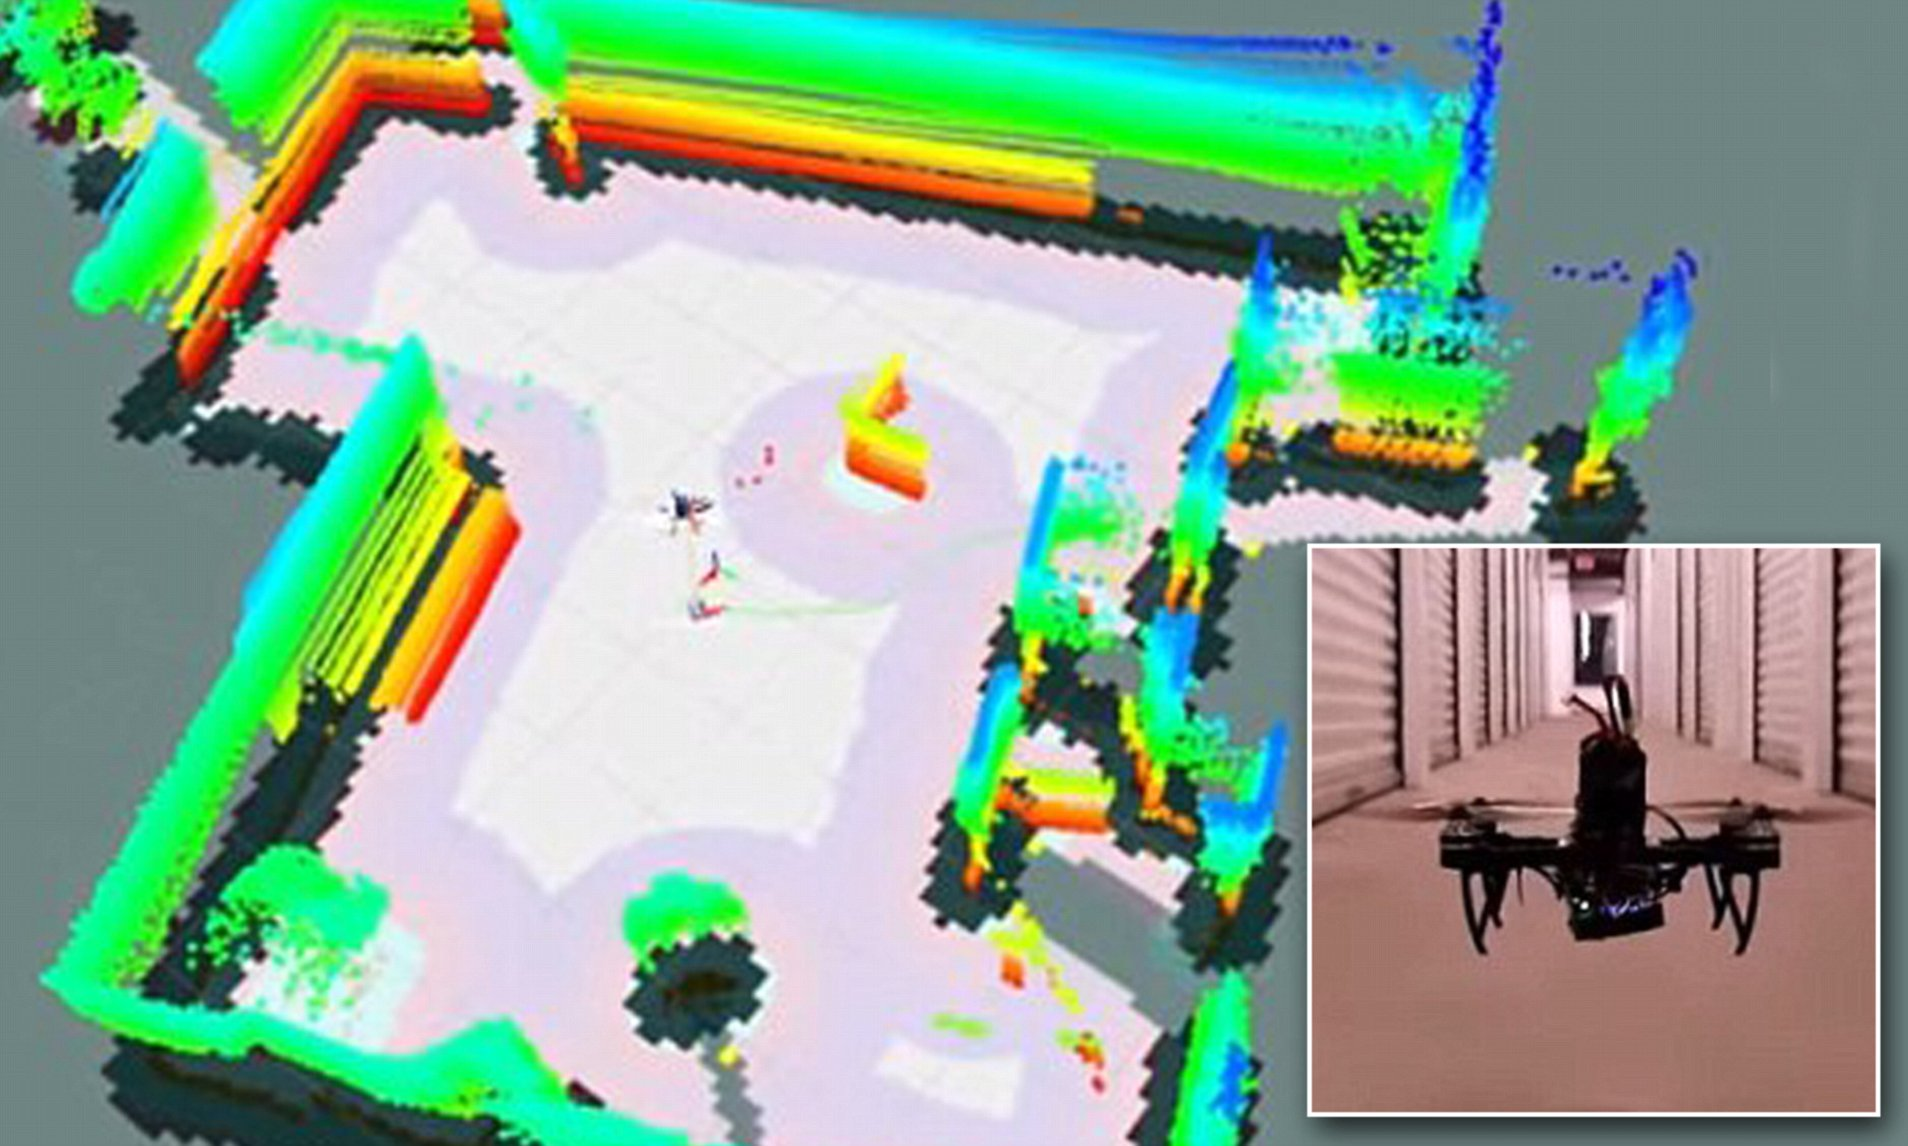
\includegraphics[width=0.6\linewidth]{drone_mapping}
  \end{figure}

  La clave es conocer su ubicación para no perderse en la exploración. Puesto que, es casi imposible para un robot operar en un ambiente sin un mapa que guíe sus movimientos, tomar desiciones y llevarlo a la tarea que se le pueda confiar.
  
\end{frame}

\begin{frame}

  Tomando la ventaja de los vehículos aéreos no tripulados en tener un punto de vista privilegiado, se vuelve interesante contar con una representación tridimencional del ambiente.
  
  \begin{figure}
    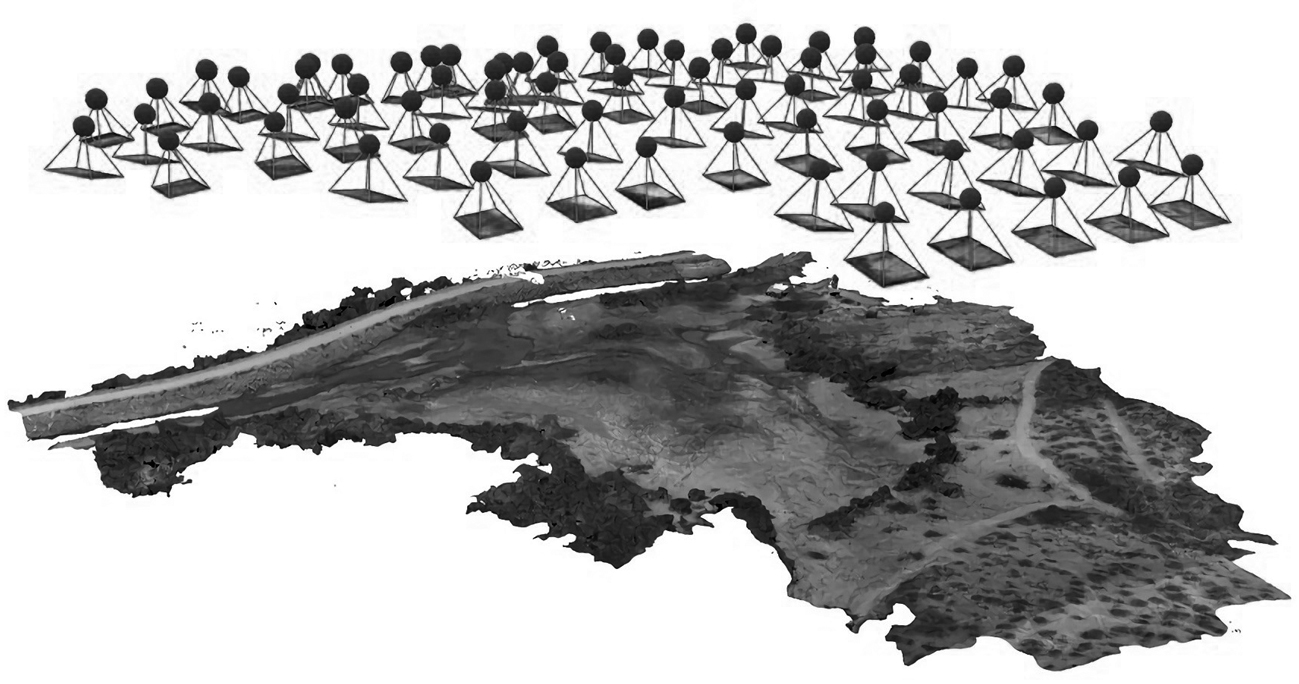
\includegraphics[width=0.7\linewidth]{drones_maps}
  \end{figure}
  
\end{frame}

\begin{frame}
  \frametitle{Aplicaciones}
  \bigskip % Vertical whitespace
  El problema de mapeo de ambientes desconocidos toma importancia en diversas aplicaciones.
  
  \begin{itemize}
  \item Búsqueda y rescate
  \item Vigilancia y seguridad
  \item Cartografía
  \item Inspecciones
  \end{itemize}
  
  \begin{figure}
    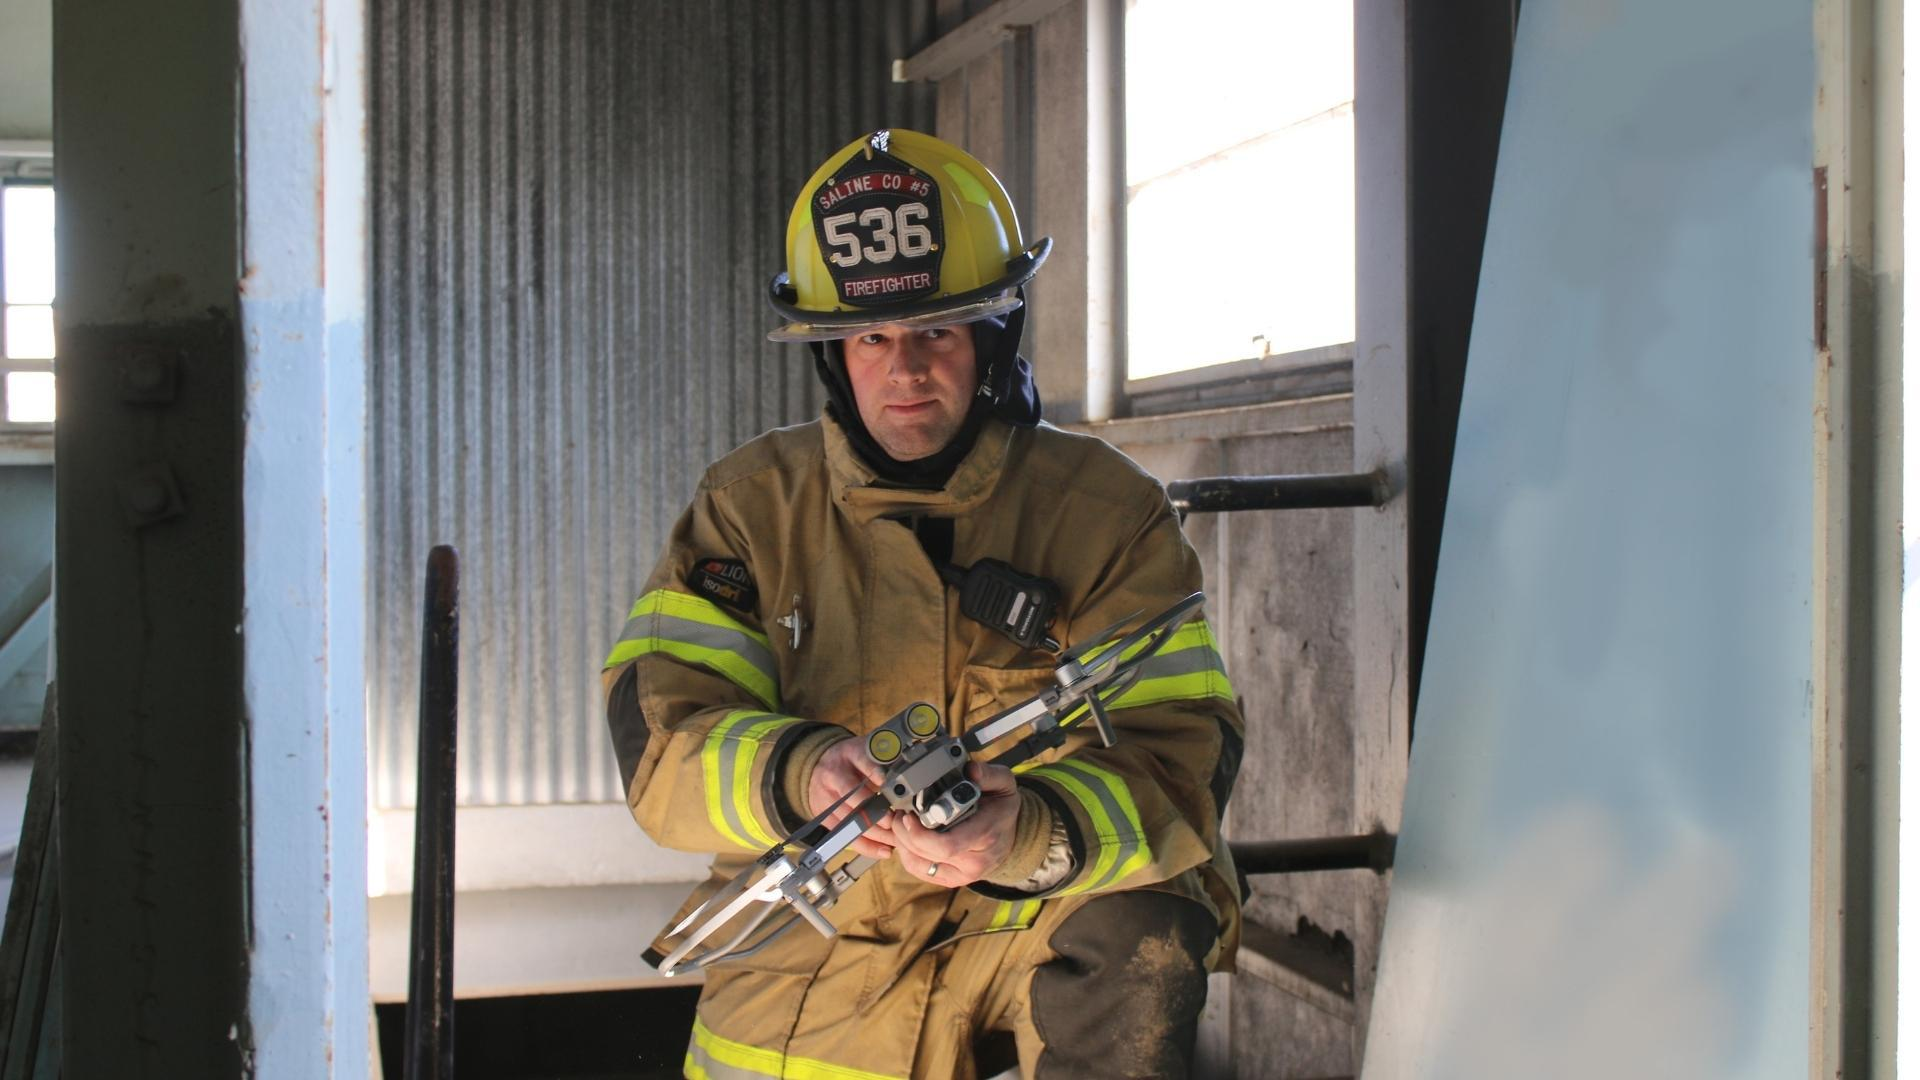
\includegraphics[width=0.5\linewidth]{search_rescue}
    \caption{Búsqueda y recate}
  \end{figure}
\end{frame}

\begin{frame}
  \begin{figure}
    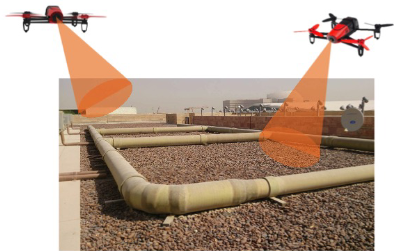
\includegraphics[width=0.7\linewidth]{pipe_inspect}
    \caption{Inspecciones}
  \end{figure}
\end{frame}



\begin{frame}
  
  Ventajas de utilizar multiples VANTs

  \begin{itemize}
  \item Capacidad de cubrir un área más amplia en menos tiempo. Cada vehículo aéreo puede ser asignado a una sección específica a explorar mediante una planificación y coordinación adecuada.
  \item Trabajo coolaborativo. Los drones pueden trabajar juntos para completar la tarea de manera eficiente
  \end{itemize}
    
  \begin{figure}
    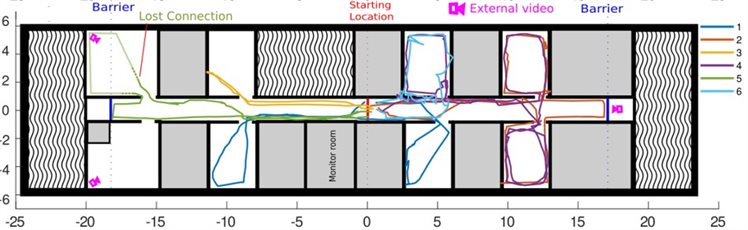
\includegraphics[width=0.7\linewidth]{drones-3.jpg}
  \end{figure}
  
\end{frame}

\begin{frame}
  Uno de los retos es la coordinación en la exploración, dicha tarea recae en la inteligencia individual de cada vehículo aéreo. Centrándonos en las habilidades de vuelo, control de velocidad y poder evadir obstáculos.

  \begin{figure}
    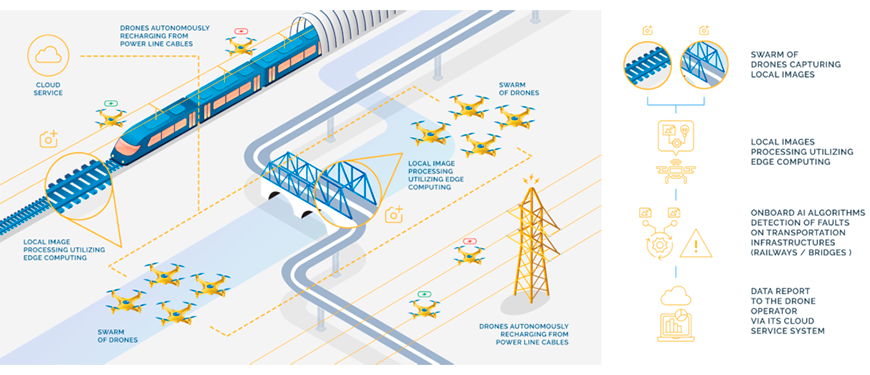
\includegraphics[width=0.9\linewidth]{drones_action}
  \end{figure}
  
  Abordar estos aspectos son importantes para lograr un desempleño óptimo.
  
\end{frame}

\begin{frame}

  Aspectos a considerar

  \begin{itemize}
  \item Rangos de comunicación entre los VANTs
  \item Tipo de arquitectura de comunicación (Centralizada, desentralizada ó distribuida). Conocer las ventajas y desventajas entre ellas
  \item Trayectorias y colisiones
  \item Cantidad de información compartida
  \end{itemize}
  
\end{frame}

\begin{frame}
  
  \begin{enumerate}
  \item Simulación - Crear algoritmos modulares. El código en el simulador, deberá ser portable a un entorno real.
  \item Creación de un drones de bajo coste DIY de código abierto con los conocimientos adquiridos. 
  \item Lograr aplicar los algoritmos en un grupo de VANTs y realizar una demostración en un ambiente controlado
  \end{enumerate}

  \begin{figure}[h]
    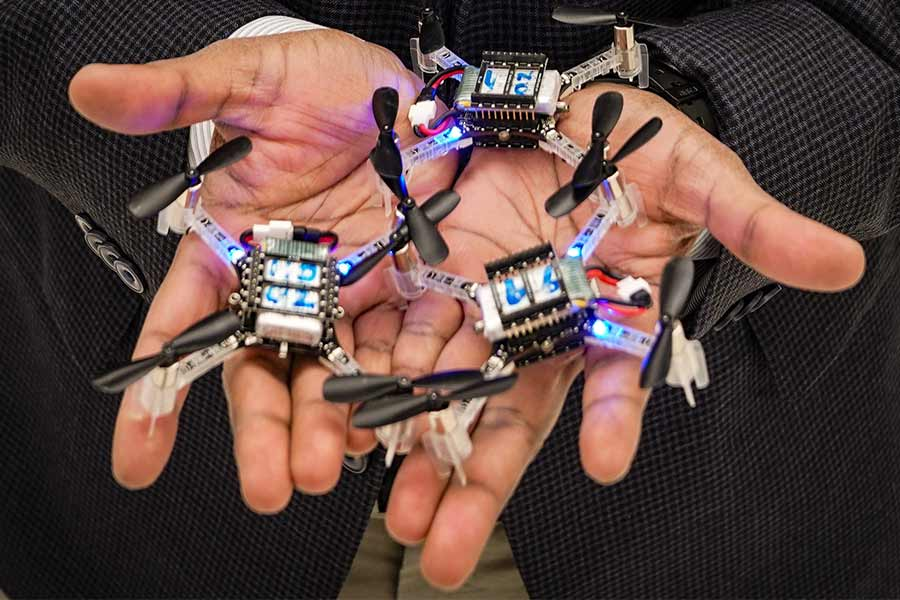
\includegraphics[width=0.5\linewidth]{drone_hand.jpg}
  \end{figure}
  
\end{frame}

\begin{frame}
  \frametitle{Simuladores}
  Antes de implementar los algoritmos en VANTs reales, probar su funcionamiento en simuladores es un paso necesario. Buscando minimizar los riesgos potenciales y gastos que puedan involucrar probar los algoritmos (Prueba y error).
  \begin{figure}
    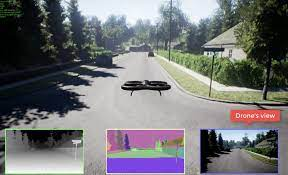
\includegraphics[width=0.5\linewidth]{airsim.jpeg}
    \caption{Airsim}
  \end{figure}
\end{frame}

\begin{frame}
  \begin{figure}
    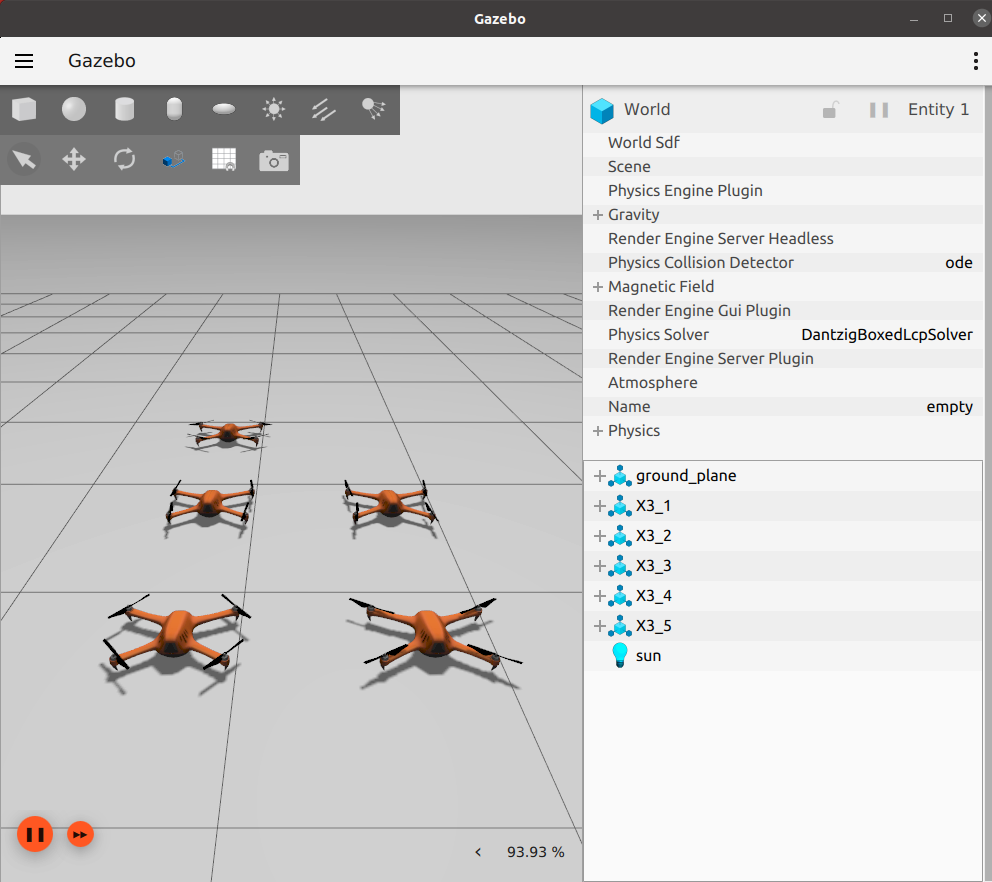
\includegraphics[width=0.7\linewidth]{gazebo.png}
    \caption{Gazebo}
  \end{figure}
\end{frame}

\begin{frame}
  \begin{figure}
    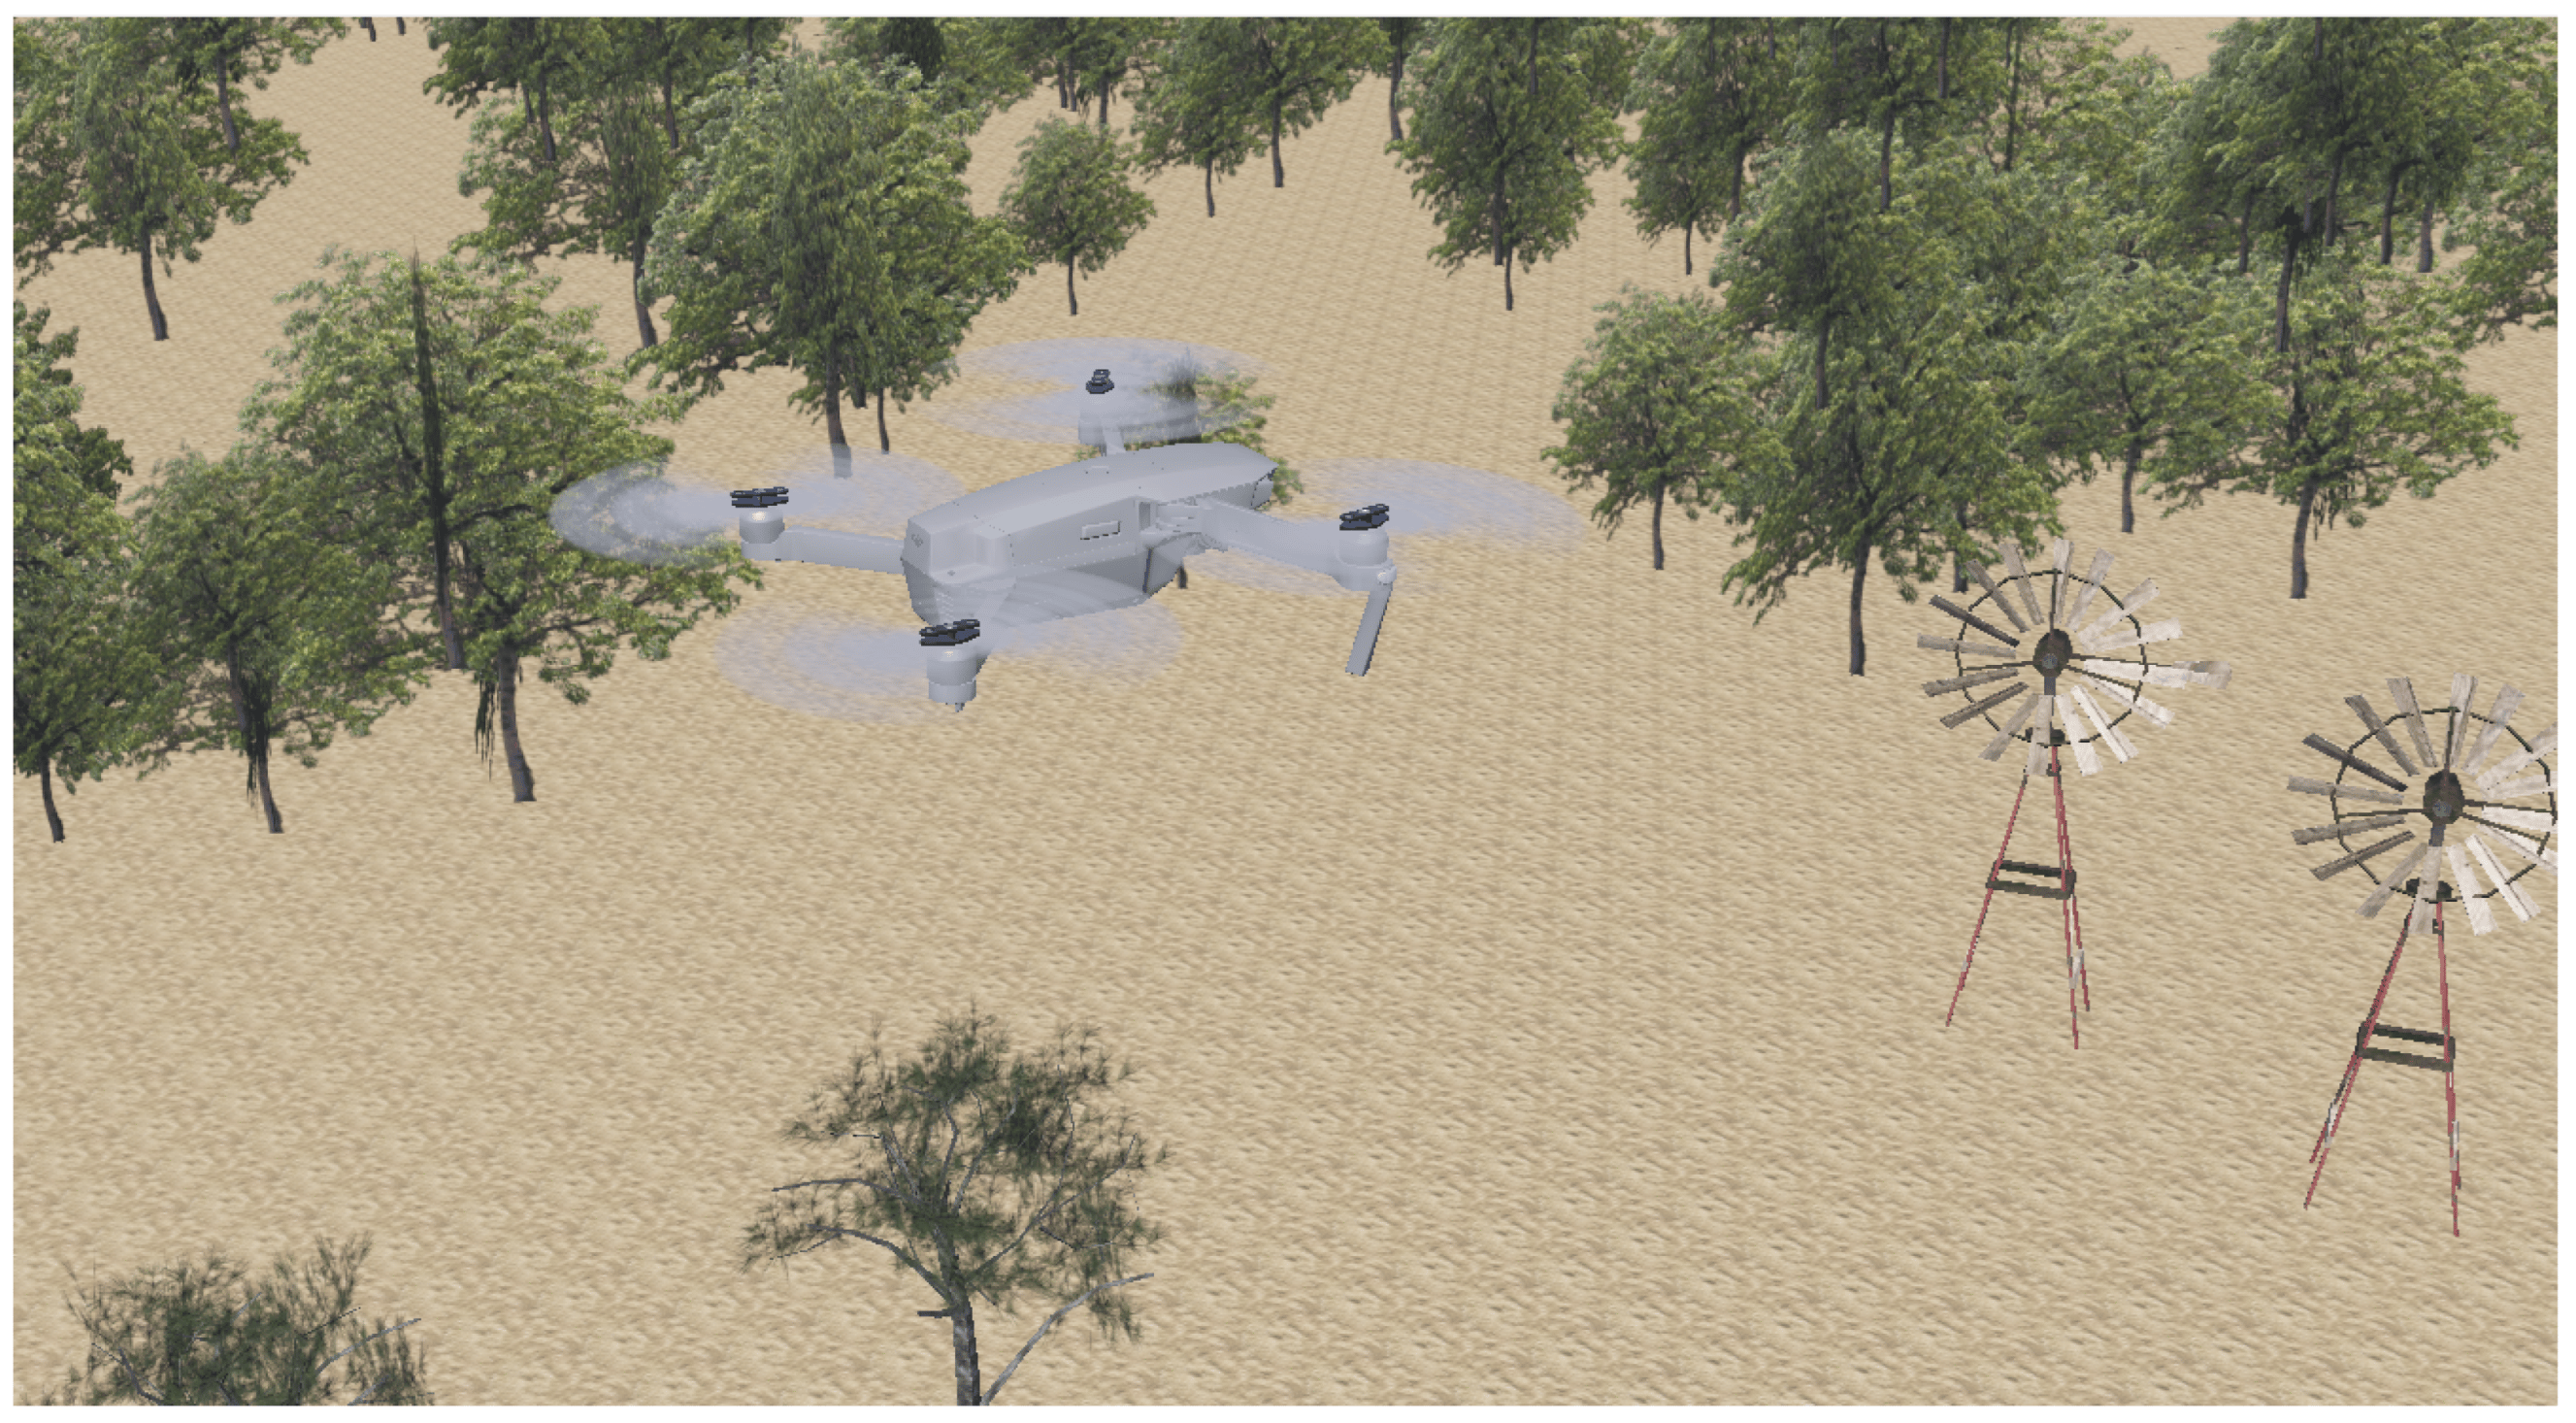
\includegraphics[width=0.7\linewidth]{webots.png}
    \caption{Webots}
  \end{figure}
\end{frame}

\begin{frame}

  \frametitle{En resumen}
  El trabajo busca brindar una propuesta novedosa para la exploración en un ambiente desconocido empleando múltiples VANTs coordinados de manera eficiente y efectiva.

  \begin{figure}[h]
    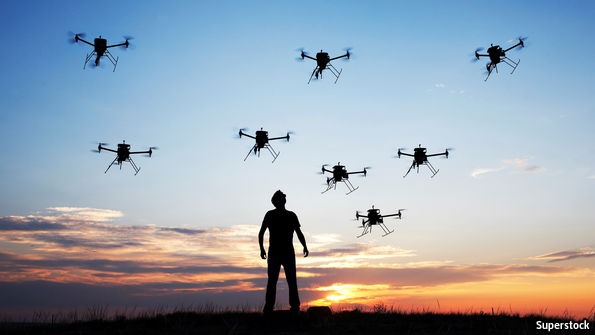
\includegraphics[width=0.7\linewidth]{swarm}
  \end{figure}
  
\end{frame}

\end{document} 
